\documentclass{article}
\usepackage[utf8]{inputenc}
\title{Statistical Inference for Entropy}
\author{Karina Marks}

\usepackage{amsmath, amsfonts, graphicx, listings, booktabs, amstext}
\usepackage[format=plain,
            textfont=it]{caption}

\newtheorem{theorem}{Theorem}
\newtheorem{remark}{Condition}

\begin{document}
\maketitle
\section{Introduction}



\section{Entropies and Properties}

Entropy can be thought of as a representation of the average information content of an observation; sometimes referred to as a measure of unpredictability or disorder. 

\subsection{Shannon Entropy}
The Shannon entropy of a random vector X with density function f is given by;
\begin{align} 
H &= - \mathbb{E} \{log(f(x))\} \nonumber \\
&= - \int_{x : f(x) > 0} f(x) log(f(x)) dx \nonumber \\
&= - \sum_{x \in \mathbb{R}^{d}} f(x) log(f(x)) \label{ShaEnt}
\end{align} 

\subsection{ R\'enyi and Tsallis Entropy}
These entropies are for the order $q \neq 1$ and the construction of them relies upon the generalisation of the Shannon entropy \ref{ShaEnt}. For a random vector $X \in \mathbb{R}^d$ with density function f, we define;

R\'enyi entropy
\begin{align} 
H_{q}^{*} &= \frac{1}{1-q} log \left( \int_{\mathbb{R}^d} f^q (x) dx \right) \quad  \quad (q \neq 1) \label{RenEnt} \\
&=  \frac{1}{1-q} log \left( \sum_{x \in \mathbb{R}^{d}} f^q (x) \right) \nonumber 
\end{align}

Tsallis entropy
\begin{align} 
H_{q} &= \frac{1}{q-1} \left(1 - \int_{\mathbb{R}^d} f^q (x) dx \right)  \quad  \quad (q \neq 1) \label{TsaEnt} \\
&=  \frac{1}{q-1} \left(1 - \sum_{x \in \mathbb{R}^d} f^q (x) \right) \nonumber 
\end{align}

When the order of the entropy $q \to 1$, both the R\'enyi, (\ref{RenEnt}), and Tsallis, (\ref{TsaEnt}), entropies tend to the Shannon entropy, (\ref{ShaEnt}), this is a special case for when $q=1$. There are also other special cases, sometimes the R\'enyi entropy is considered for the special case, $q=2$, and known as the quadratic R\'enyi entropy;
\begin{align} 
H_{2}^{*} &= - log\left( \int_{\mathbb{R}^{d}} f^2(x) dx \right) \label{QuadRenEnt} \\
&= - log \left( \sum_{x \in \mathbb{R}^d} f^2 (x) \right) \nonumber 
\end{align}
As $q \to \infty$, the limit of the R\'enyi entropy exists, and is defined as the minimum entropy, since it's the smallest possible value of $H_{q}^{*}$;
\begin{equation}
H_{\infty}^{*} = - \log \sup_{x \in \mathbb{R}^d} f (x) \nonumber
\end{equation}
Thus, it follows that; $H_{\infty}^{*} \leq H_{2}^{*} \leq 2H_{\infty}^{*}$.

There is also an approximate relationship between the Shannon entropy and the quadratic R\'enyi entropy;
\begin{equation}
H_{2}^{*} \leq H \leq \log(d) + \frac{1}{d} - e^{-H_{2}^{*}} \nonumber
\end{equation}
where $H_{2}^{*}$ is the quadratic R\'enyi entropy (\ref{QuadRenEnt}), H is the Shannon entropy (\ref{ShaEnt}) and d is the dimension of the distribution.

\section{Estimation of Entropy}

\subsection{Kozachenko-Leonenko Estimator}

We now wish to introduce the Kozachenko-Leonenko estimator of the entropy H. Let $X_{1}, X_{2}, ... ,X_{N}$, $N \geq 1$ be independent and identically distributed random vectors in $\mathbb{R}^{d}$, and denote $\|.\|$ the Euclidean norm on $\mathbb{R}^{d}$.
 
\begin{itemize}

\item For $i = 1, 2, ..., N$, let $X_{(1), i}, X_{(2), i}, .., X_{(N-1), i}$ denote an order of the $X_{k}$ for $k = \{1, 2, ..., N\} \setminus \{i\}$, such that $\| X_{(1), i} - X_{i}\| \leq \cdots \leq \|  X_{(N-1), i} - X_{i}\| $. Let the metric $\rho$, defined as;
\begin{equation} \label{Rho}
\rho_{(k), i} = \| X_{(k), i} - X_{i}\|
\end{equation} denote the kth nearest neighbour or $X_{i}$.

\item  For dimension d, the volume of the unit d-dimensional Euclidean ball is defined as;
\begin{equation} \label{Volume}
V_{d} = \frac{\pi^\frac{d}{2}}{\Gamma(1 + \frac{d}{2})}
\end{equation}

\item For the kth nearest neighbour, the digamma function is defined as;
\begin{equation} \label{Psi}
\Psi(k) = -\gamma + \sum_{j=1}^{k-1} \frac{1}{j}
\end{equation}
where $\gamma = 0.577216$ is the Euler-Mascheroni constant (where the digamma function is chosen so that $\frac{e^{\Psi(k)}}{k}\to1$ as $k \to \infty$).

\end{itemize} Then the Kozachenko-Leonenko estimator for entropy, H, is given by;
\begin{equation} \label{KLest}
\hat{H}_{N, k} = \frac{1}{N} \sum_{i=1}^{N} log \left[ \frac{\rho_{(k),i}^{d} V_{d} (N-1)}{e^{\Psi(k)}} \right]
\end{equation} where, $\rho_{(k),i}^{d}$ is defined in (\ref{Rho}), $V_{d}$ is defined in (\ref{Volume}) and $\Psi(k)$ is defined in (\ref{Psi}).This estimator for entropy, when $d \leq 3$, under a wide range of k and some regularity conditions, satisfies some  theorems. Firstly from PAPER 1 (TODO refrence), we have the following;

\begin{theorem} \label{paper1_T1}
For exact entropy $H$, Kozachenko-Leonenko estimator $\hat{H}_{N,k}$, and density function $f(x)$, for some $\epsilon > 0$ if both
\begin{equation} \label{paper1_T1_eq1}
\int_{\mathbb{R}^{d}} | log(f(x))|^{1 + \epsilon} f(x) dx < \infty 
\end{equation}
and
\begin{equation} \label{paper1_T1_eq1}
\int_{\mathbb{R}^{d}} \int_{\mathbb{R}^{d}} | log(\|x-y\|)|^{2+ \epsilon} f(x) f(y) dx dy < \infty
\end{equation}
Then we have that 
\begin{equation} 
\lim_{N \to \infty} \mathbb{E} (\hat{H}_{N, k}) = H \nonumber
\end{equation}
Thus $\hat{H}_{N, k}$ is an asymptotically unbiased estimator of $H$.
\end{theorem}

\begin{theorem} \label{paper1_T2}
For exact entropy $H$, Kozachenko-Leonenko estimator $\hat{H}_{N,k}$, and density function $f(x)$, for some $\epsilon > 0$ if both
\begin{equation}
\int_{\mathbb{R}^{d}} | log(f(x))|^{2 + \epsilon} f(x) dx < \infty \nonumber
\end{equation}
and
\begin{equation}
\int_{\mathbb{R}^{d}} \int_{\mathbb{R}^{d}} | log(\|x-y\|)|^{2+ \epsilon} f(x) f(y) dx dy < \infty \nonumber
\end{equation}
Then $\hat{H}_{N, k}$ for $N \to \infty$ is a consistent estimator of H.

(An estimator is consistent if the probability that it is in error by more than a given amount tends to zero as the sample become large $\Leftrightarrow $ for error $\delta > 0$, we have $\lim_{N \to \infty} \mathbb{P}(|\hat{H}_{N,k} - H| < \delta) = 1$) 
\end{theorem}

Additionally, from paper 4 (TODO reference), we have the following, stronger conditions which will be used in Theorems \ref{paper4_T4} and \ref{paper4_T5};
\begin{remark} ($\beta$) \label{A1}
For density $f$ bounded, denoting $m := \lfloor \beta \rfloor$ and $\eta := \beta -m$, we have that $f$ is $m$ times continuously differentiable and there exists $r_{*} > 0$ and a Borel measurable function $g_{*}$ such that for each $t = 1, 2, ... , m$ and $\|y-x\| \leq r_{*}$, we have;
\begin{equation}
\| f^{(t)} (x) \| \leq g_{*}(x)f(x) \nonumber
\end{equation},
\begin{equation}
\| f^{(m)} (y) - f^{(m)} (x) \| \leq g_{*}(x)f(x) \|y-x\|^{\eta} \nonumber
\end{equation}
and $sup_{x:f(x)\geq \delta} g_{*}(x) = o(\delta^{-\epsilon})$ as $\delta \downarrow 0$, for each $\epsilon > 0$.
\end{remark}

\begin{remark} ($\alpha$) \label{A2}
For density $f(x)$ and dimension $d$, we have;
\begin{equation}
\int_{\mathbb{R}^{d}} \| x \|^{\alpha} f(x) dx < \infty \nonumber
\end{equation}
\end{remark}

\begin{remark} \label{A3}
Assume that condition \ref{A1} holds for $\beta = 2$ and condition \ref{A2} holds for some $\alpha > d$. Let $k_{0}^{*} = k_{0, N}^{*}$ and $k_{1}^{*} = k_{1, N}^{*}$ denote two deterministic sequences of positive integers with $k_{0}^{*} \leq k_{1}^{*}$, with $\frac{k_{0}^{*}}{\log^{5}{N}} \to 0$ and with $k_{1}^{*} = O(N^{\tau})$, where
\begin{equation}
\tau < \min \left\{ \frac{2 \alpha}{5 \alpha + 3d} , \frac{\alpha - d}{2 \alpha} , \frac{4}{4 + 3d} \right\} \nonumber
\end{equation}
\end{remark}

\begin{theorem}\label{paper4_T4}
Assume that condition \ref{A1} holds for $\beta = 2$ and condition \ref{A2} holds for some $\alpha > d$, then by condition \ref{A3}, for the estimator $\hat{H}_{N, k}$ we have;
\begin{equation}
Var(\hat{H}_{N, k}) = \frac{Var(\log f(x))}{N} + o(\frac{1}{N}) \nonumber
\end{equation}
as $N \to \infty$, uniformly for $k \in \{ k_{0}^{*}, ...,  k_{1}^{*} \}$.
\end{theorem}

\begin{theorem} \label{paper4_T5}
Assume that $d \leq 3$ and the conditions of Theorem \ref{paper4_T4} are satisfied (where if $d=3$, we additionally assume $k_{1}^{*} = o(n^{\frac{1}{4}})$. Then, for the estimator $\hat{H}_{N, k}$ we have;
\begin{equation} \label{est_dist}
\sqrt{N}(\hat{H}_{N, k} - H) \xrightarrow{d} N(0, \sigma^2)
\end{equation}
and 
\begin{equation} \label{est_consist}
N \mathbb{E}{(\hat{H}_{N, k} - H)^2} \xrightarrow{} \sigma^2
\end{equation}
as $N \to \infty$ uniformly for $k \in \{ k_{0}^{*}, ...,  k_{1}^{*} \}$, where $\sigma^2 = Var(log(f(x))$, for density function $f(x)$.

(This combines Theorem \ref{paper1_T1} with stronger conditions; hence we can now say that $\hat{H}_{N, k}$ is an consistent and asymptotically unbiased estimator of exact entropy $H$.)
\end{theorem}

Theorem \ref{paper4_T5} holds, according to the central limit theorem, on the estimator for entropy $\hat{H}_{N, k}$;
\begin{equation}
\frac{\hat{H}_{N, k} - \mathbb{E}{\hat{H}_{N, k}}}{\sqrt{Var(\hat{H}_{N, k})}} \xrightarrow{d} N(0, \sigma^2) \nonumber
\end{equation}
By Theorem \ref{paper4_T4}, we can assume that $Var(\hat{H}_{N, k}) = \frac{Var(\log f(x))}{N} \approx \frac{1}{N}$, as for large $N$, the variance of the logarithm of the density function stays constant. Thus, the left side of the central limit theorem above can be written as;
\begin{align*}
\frac{\hat{H}_{N, k} - \mathbb{E}{\hat{H}_{N, k}}}{\sqrt{Var(\hat{H}_{N, k})}} &= \sqrt{N}(\hat{H}_{N, k} - \mathbb{E}{\hat{H}_{N, k}}) \\
&= \sqrt{N}[(\hat{H}_{N, k} - H) + (H - \mathbb{E}{\hat{H}_{N, k}})] \\
&= \sqrt{N}(\hat{H}_{N, k} - H) + \sqrt{N}(H - \mathbb{E}{\hat{H}_{N, k}})
\end{align*}
and as $N \to \infty$ this tends to the normal distribution, $N(0, \sigma^2)$. So we can say that $\sqrt{N}(\hat{H}_{N, k} - H) \xrightarrow{d} N(0, \sigma^2)$ while $\sqrt{N} (H - \mathbb{E}{\hat{H}_{N, k}}) \to \sigma^2$, which is equivalent to the properties stated in Theorem \ref{paper4_T5}.

Later, I will further discuss this estimator for the specific dimensions $d=1$ and $d=2$; however, it is important to note that for larger dimensions this estimator is not accurate. When $d=4$, equations (\ref{est_dist}) and (\ref{est_consist}) no longer hold but the estimator $\hat{H}_{N, k}$, defined by (\ref{KLest}), is still root-N consistent, provided k is bounded. Also, when $d \geq 5$ there is a non trivial bias, regardless of the choice of $k$. There is a new proposed estimator, formed as a weighted average of $\hat{H}_{N, k}$ for different values of $k$, where $k$ depends on the choice of $N$, explored in PAPER 4 (TODO reference). 

Moreover, this paper focuses only on distributions for $d \leq 3$, more specifically, I will first be considering samples from 1-dimensional distributions, $d=1$. Therefore, the volume of the 1-dimensional Euclidean ball is given by $V_{1} = \frac{\pi^{\frac{1}{2}}}{\Gamma (\frac{3}{2})} = \frac{\sqrt{\pi}}{\frac{\sqrt{\pi}}{2}} = 2$. Hence the Kozachenko-Leonenko estimator is of the form;
\begin{equation} \label{KLest_d=1}
\hat{H}_{N, k} = \frac{1}{N} \sum_{i=1}^{N} log \left[ \frac{2\rho_{(k),i}(N-1)}{e^{\Psi(k)}} \right]
\end{equation}
 Later, I will be considering samples from 2-dimensional distributions; thus, $d=2$ and the volume of the 2-dimensional Euclidean ball is given by $V_{2} = \frac{\pi^{\frac{2}{2}}}{\Gamma (2)} = \frac{\pi}{1} = \pi$. Hence, the estimator takes the form;
\begin{equation} \label{KLest_d=2}
\hat{H}_{N, k} = \frac{1}{N} \sum_{i=1}^{N} log \left[ \frac{\pi \rho_{(k),i}^{2} (N-1)}{e^{\Psi(k)}} \right]
\end{equation}



\subsection{Other Estimators}
\begin{itemize}
\item The estimator for $H_{2}^{*}$ from paper 5
\item The estimator for higher dimensions $d$, from paper 4
\end{itemize}



\section{Monte-Carlo Simulations}

In this section I will explore simulations of the bias of estimator (\ref{KLest}) in comparison to the size of the sample estimated from, with respect to different values of k; firstly exploring 1-dimensional distributions and then progressing onto 2-dimensional.

The motivation for these simulations is to explore the consistency of this estimator for different values of $k$; the relationship between the size of the bias of the estimator $\hat{H}_{N, k}$, $Bias(\hat{H}_{N, k})$,  and the sample size, $N$. Throughout this analysis we will be considering the absolute value of this bias, since when considering its logarithm, we need a positive value. Using Theorem \ref{paper4_T5}, we can write that the bias of the estimator approaches 0 as $N \to \infty$. This is because we can write $Bias(\hat{H}_{N, k} ) = \mathbb{E}(\hat{H}_{N, k}) - H$, which in equation (\ref{est_consist}) implies $Bias(\hat{H}_{N, k}) \to 0$ as $N \to \infty$. Thus, there must be a type of inverse relationship between the modulus of the bias of the estimator, $|Bias(\hat{H}_{N, k})|$, and $N$. We believe this relationship is of the form;
\begin{equation} \label{bias}
|Bias(\hat{H}_{N, k})| = \frac{c}{N^a}
\end{equation}
for $a, c > 0$. By taking the logarithm of this, we can generate a linear relationship, which is easier to analyse, and is given by;
\begin{equation} \label{logbias}
log|Bias(\hat{H}_{N, k})| = log(c) - a [log(N)]
\end{equation}
I will investigate the consistency of this estimator for a sample from the normal distribution, dependent on the value of $k$, this mean finding the optimum value of $k$ for which $|Bias(\hat{H}_{N, k})| \to 0$ for $N \to \infty$. For the relationship in equation (\ref{bias}), this will happen for large values of $a$ and relatively small $c$, as $N \to \infty$. Moreover, I wish to also examine the dependence of $c$ on the value of $k$. As I wish to consider the difference in accuracy of the estimator when using different values of k, let us denote the approximate values for $a$ and $c$ dependent on $k$ as $a_{k}$ and $c_{k}$.


\subsection{1-dimensional Normal Distribution} \label{Normal_d=1}
I will begin by exploring entropy of samples from the normal distribution $N(0, \sigma^2)$, where without loss of generality we can use the mean $\mu = 0$ and change the variance $\sigma^2$ as needed. The normal distribution has an exact formula to work out the entropy, given the variance $\sigma^2$. Using equation (\ref{ShaEnt}) and the density function for the normal distribution $f(x) = \frac{1}{\sqrt{(2\pi)} \sigma}\exp{ \left( \frac{-x^2}{2\sigma^2} \right)}$ for $x \in \mathbb{R}$, given $\mu = 0$. We can write the exact entropy for the normal distribution, using equation (\ref{ShaEnt});
\begin{align}
H &= - \int_{x : f(x) > 0} f(x) log(f(x)) dx \nonumber \\
&= - \int_{\mathbb{R}} \frac{1}{\sqrt{(2\pi)} \sigma}\exp{ \left( \frac{-x^2}{2\sigma^2} \right)} log \left[\frac{1}{\sqrt{(2\pi)} \sigma}\exp{ \left( \frac{-x^2}{2\sigma^2} \right)} \right] dx \nonumber \\
&=  \int_{\mathbb{R}} \frac{1}{\sqrt{(2\pi)} \sigma}\exp{ \left( \frac{-x^2}{2\sigma^2} \right)} \left( log(\sqrt{(2\pi)}\sigma) +  \frac{x^2}{2\sigma^2} \right) \nonumber \\
&= \frac{log(\sqrt{(2\pi)}\sigma)}{\sqrt{(2\pi)} \sigma} \int_{\mathbb{R}} \exp{ \left( \frac{-x^2}{2\sigma^2} \right)} dx +  \frac{1}{2\sqrt{(2\pi)} \sigma} \int_{\mathbb{R}} \frac{x^2}{2\sigma^2}  \exp{ \left( \frac{-x^2}{\sigma^2} \right)} dx \nonumber \\
&=  log(\sqrt{(2\pi)}\sigma) + \frac{1}{2} \nonumber 
\end{align}
Thus the exact entropy for the normal distribution is given by 
\begin{equation}\label{NormalEnt}
H =  log(\sqrt{(2\pi e)}\sigma) 
\end{equation}

The normal distribution satisfies Theorem \ref{paper1_T1} because the density function is given by $f(x) = C \exp{ \left( \frac{-x^2}{2\sigma^2} \right)}$ for $x \in \mathbb{R}$, given $\mu = 0$ and where $C:= \frac{1}{\sqrt{(2\pi)} \sigma} > 0$. Then by equation (\ref{paper1_T1_eq1}), considering that here $d=1$ we have;
\begin{align}
\int_{\mathbb{R}} | log(f(x))|^{1 + \epsilon} f(x) dx  &= \int_{\mathbb{R}} \left| log\left( C\exp{ \left( \frac{-x^2}{2\sigma^2} \right)} \right) \right|^{1 + \epsilon}C\exp{ \left( \frac{-x^2}{2\sigma^2} \right)} dx \\ \nonumber
&= C \int_{\mathbb{R}} \left| log \left( C \right) -  \left( \frac{x^2}{2\sigma^2} \right) \right|^{1 + \epsilon} \exp{ \left( \frac{-x^2}{2\sigma^2} \right)} dx \\ \nonumber
&\approx \int_{-\infty}^{\infty} \frac{x^{\epsilon}}{ \exp{x^2}} dx \\ \nonumber
&< \infty
\end{align}





I will first explore the 1-dimensional standard normal distribution with mean $\mu = 0$ and variance $\sigma^2 = 1$, $N(0, 1)$. The exact entropy of this distribution is given by;
\begin{equation} \label{normal_exact}
H = log(\sqrt{(2\pi e)}) \approx 1.418939
\end{equation}

Since, I am first considering the 1-dimensional normal distribution, the Kozachenko-Leonenko estimator takes the form in equation (\ref{KLest_d=1});
\begin{equation}
\hat{H}_{N, k} =  \frac{1}{N} \sum_{i=1}^{N} log \left[ \frac{2\rho_{(k),i}(N-1)}{e^{\Psi(k)}} \right]\nonumber
\end{equation}




\subsubsection{k=1} \label{N_k=1}
I will be considering k=1 for the estimator of entropy; thus, the estimator will take the form;
\begin{equation} 
\hat{H}_{N, 1} = \frac{1}{N} \sum_{i=1}^{N} log \left[ \frac{2\rho_{(1),i} (N-1)}{e^{\Psi(1)}} \right] = \frac{1}{N} \sum_{i=1}^{N} log \left[ \frac{2\rho_{(1),i} (N-1)}{e^{-\gamma}} \right] \nonumber
\end{equation}

I will consider $500$ samples of size $N$ from this distribution, find the estimator in each case and take the average of these estimators to find our entropy estimator, shown in table \ref{normal_k=1_table}. We will then consider the relationship show in (\ref{logbias}) for each sample and again work out the average for the values of a and c, shown in \ref{normal_k=1_graph}.

\begin{table}
\caption{1-dimensional normal distribution, $k=1$} \label{normal_k=1_table}
\begin{center}
\begin{tabular}{| l | c c c|} 
\toprule
$N$ & $\hat{H}_{N, 1}$ & $|Bias(\hat{H}_{N, 1})|$ & $Var(Bias(\hat{H}_{N, 1}))$ \\
\midrule[1pt]
100     & 1.405890     & 0.01304883282     & 0.0275142086  \\
200     & 1.411070     & 0.00786872927     & 0.0128689734  \\
500     & 1.416666     & 0.00227293433     & 0.0051416433  \\
1000    & 1.419401     & 0.00046261516     & 0.0028127916  \\
5000    & 1.418469     & 0.00046981107     & 0.0005147810  \\
10000   & 1.417998     & 0.00094067533     & 0.0002472848  \\
25000   & 1.418877     & 0.00006147045     & 0.0001088641  \\
50000   & 1.419286     & 0.00034705584     & 0.0000496450  \\
\hline
\end{tabular}
\end{center}
\end{table}

Considering table \ref{normal_k=1_table}, we can see for a larger value of N, the Bias of the estimator becomes much smaller; the bias decreases from $\approx 0.0130$ to $\approx 0.0003$ as $N$ increases from $100 \to 50,000$. This result is to be expected for an estimator to satisfy the consistency condition, shown in Theorem \ref{consistency_theorem}. We can also see that the variance of the bias is decreasing as N increases implying that, not only is the average of the estimator getting closer to the actual value of entropy, also the variability between the estimator of different samples is decreasing, making it a consistent and asymptotically unbiased estimator in practice, as well as in theory.

This relationship between the bias $|Bias(\hat{H}_{N, 1})|$ of the estimator and the size of the sample $N$, can be computed for these sample sizes. Figure \ref{normal_k=1_graph}, shows this relationship of $log|Bias(\hat{H}_{N, 1})|$ against $log(N)$ with a fitted regression line. In this graph, I have considered the values of $N$ up to $50,000$ at intervals of size $100$, where each point is calculate $500$ times and the average estimator is plotted. I have also found the corresponding coefficients $a_{1}$ and $c_{1}$ for the relationship shown in (\ref{bias}). These coefficients tend towards $a_{1} = 0.4594$ and $c_{1} = 0.0249$ for a large $N$; 
\begin{table}
\begin{center}
\begin{tabular}{| l | c c|}
\toprule
$N$ & $a_{1}$ & $c_{1}$ \\
\midrule[1pt]
5000   &  0.6545   &   0.1845   \\
75000 &  0.5011   &   0.0462   \\
10000 &  0.7699   &   0.3512   \\
25000 &  0.5442   &   0.0620   \\
50000 &  0.4594   &   0.0249   \\
\end{tabular}
\end{center}
\end{table}

Doesn't show what expected.. TODO..

\begin{equation}
|Bias(\hat{H}_{N, 1})| \approx \frac{0.0249}{N^{0.4594}} \nonumber
\end{equation}
On their own these coefficients show that there is a negative relationship between $log(|Bias(\hat{H}_{N, 1})|)$ and $log(N)$. This implies that the relationship between the Bias and N is such that as N increases the Bias decreases to 0. Hence, creating a consistent estimator for entropy, when considering the 1-dimensional normal distribution with k=1 in the Kozachenko-Leonenko estimator. However, to understand better the meaning of this relationship we must compare this to coefficients found of the regression relationships for different values of $k$, and for different distributions.

\begin{figure}
  \begin{center}
    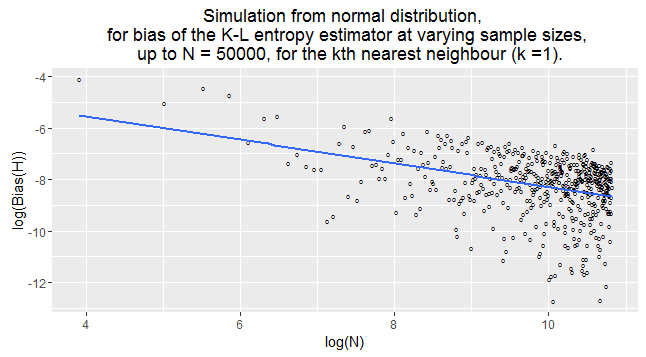
\includegraphics[width=\textwidth]{./Graphs/Normal_k=1_plot.png}
  \end{center}
\caption{Regression plot of $\log|Bias(\hat{H}_{N, 1})|$ against $\log(N)$}
  \label{normal_k=1_graph}
\end{figure}




\subsubsection{k=2} \label{N_k=2}
I am now going to examine the case where k=2 in the Kozachenko-Leonenko estimator, to compare the results of simulations from this estimator with that for k=1. Here the estimator will take the form;
\begin{equation}
\hat{H}_{N, 2} = \frac{1}{N} \sum_{i=1}^{N} log \left[ \frac{2\rho_{(2),i} (N-1)}{e^{\Psi(2)}} \right] = \frac{1}{N} \sum_{i=1}^{N} log \left[ \frac{2\rho_{(2),i} (N-1)}{e^{-\gamma + 1}} \right] \nonumber
\end{equation}

I wish to explore, in a similar manner as for k=1, the changes in the bias of the estimator depending on a change in N. Additionally, later I will make the comparison between the regression coefficients for different values of k. I will again consider 500 samples of size N from the 1-dimensional standard normal distribution $N(0, 1)$, the results from the analysis is shown in table \ref{normal_k=2_table}.

\begin{table}
\caption{1-dimensional normal distribution, $k=2$} \label{normal_k=2_table}
\begin{center}
\begin{tabular}{| l | c c c|} 
\toprule
$N$ & $\hat{H}_{N, 2}$ & $|Bias(\hat{H}_{N, 2})|$ & $Var(Bias(\hat{H}_{N, 2}))$ \\
\midrule[1pt]
100     & 1.408856     & 0.0100827948     & 0.01357417708  \\
200     & 1.411165     & 0.0077730666     & 0.00688250329  \\
500     & 1.419158     & 0.0002199163     & 0.00296693934  \\
1000    & 1.415719     & 0.0032197158     & 0.00141616592  \\
5000    & 1.418236     & 0.0007026416     & 0.00028872533  \\
10000   & 1.418656     & 0.0002824567     & 0.00014348493  \\
25000   & 1.418376     & 0.0005620780     & 0.00005791073  \\
50000   & 1.418681     & 0.0002574343     & 0.00002956529  \\
\hline
\end{tabular}
\end{center}
\end{table}

We can see that, as expected, the Bias of the estimator decreases from $\approx 0.0100$ when $N=100$ to $\approx 0.0002$ when $N=50,000$. This is showing that the consistency condition is being met since as $N \to \infty$ we have $|Bias(\hat{H}_{N, 2})| \to 0$, which is equivalent to saying $\lim_{N \to \infty} \mathbb{E} (\hat{H}_{N, k}) = H$, Theorem (\ref{consistency_theorem}). We also have that the variance of the bias of these estimators decrease as $N \to \infty$, as expected. In relation to $k=1$, we can see that the bias of this estimator for $k=2$ decreases at a similar pace as $N \to \infty$; $|Bias(\hat{H}_{N, 1})| \approx 0.0130 \to 0.0003$ and $|Bias(\hat{H}_{N, 2})| \approx 0.0101 \to 0.0002$, implying that from this analysis we cannot decide which value of $k$ generates a better estimator.

\begin{figure}
  \begin{center}
    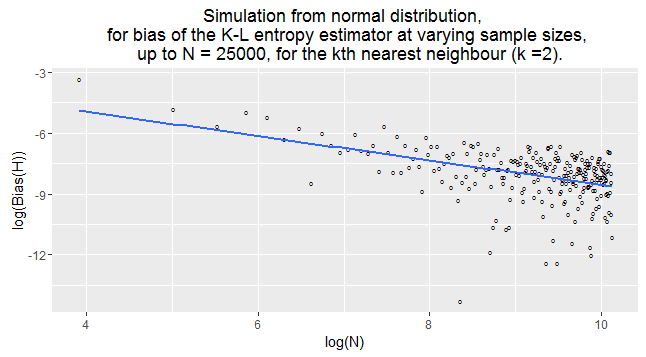
\includegraphics[width=\textwidth]{./Graphs/Normal_k=2_plot.png}
  \end{center}
\caption{Regression plot of $\log|Bias(\hat{H}_{N, 2})|$ against $\log(N)$}
  \label{normal_k=2_graph}
\end{figure}

We have found the coefficients for the equation (\ref{bias}), for $k=2$, which are given by $a_{2} = 0.5998$ and $c_{2} = 0.0746$, thus;
\begin{equation}
|Bias(\hat{H}_{N, 2})| \approx \frac{0.0746}{N^{0.5998}} \nonumber
\end{equation}

Again, this shows the relationship one would expect, that $|Bias(\hat{H}_{N, 2})| \to 0$ as $N \to \infty$. This relationship for $k=2$ is stronger than that for $k=1$ since $a_{1} \leq a_{2}$. A full comparison of the relationship of $|Bias(\hat{H}_{N, 1})|$ to $N$ and $|Bias(\hat{H}_{N, 2})|$ to $N$ is given in section \ref{N_compare_k}.




\subsubsection{k=3} \label{N_k=3}
Again, for $k=3$, I will examine $500$ samples of size $N$ from the standard normal distribution considered before; with estimator of the form;
\begin{equation}
\hat{H}_{N, 3} = \frac{1}{N} \sum_{i=1}^{N} log \left[ \frac{2\rho_{(3),i} (N-1)}{e^{\Psi(3)}} \right] = \frac{1}{N} \sum_{i=1}^{N} log \left[ \frac{2\rho_{(3),i} (N-1)}{e^{-\gamma + 1 + \frac{1}{2}}} \right] \nonumber
\end{equation}

\begin{table}
\caption{1-dimensional normal distribution, $k=3$} \label{normal_k=3_table}
\begin{center}
\begin{tabular}{| l | c c c|} 
\toprule
$N$ & $\hat{H}_{N, 3}$ & $|Bias(\hat{H}_{N, 3})|$ & $Var(Bias(\hat{H}_{N, 3}))$ \\
\midrule[1pt]
100     & 1.398784     & 0.0201546812     & 0.01210622150  \\
200     & 1.412908     & 0.0060302660     & 0.00530612702  \\
500     & 1.414035     & 0.0049035937     & 0.00223855589  \\
1000    & 1.416105     & 0.0028340080     & 0.00107754839  \\
5000    & 1.420184     & 0.0012459298     & 0.00022320970  \\
10000   & 1.418351     & 0.0005874791     & 0.00011630350  \\
25000   & 1.419115     & 0.0001760980     & 0.00004286406  \\
50000   & 1.418853     & 0.0000851863     & 0.00002257717  \\
\hline
\end{tabular}
\end{center}
\end{table}

The results of the comparison between the actual value and the estimated value of entropy, for different values of $N$, are displayed in table \ref{normal_k=3_table}. This shows again, that the Kozachenko-Leonenko estimator for entropy, $\hat{H}_{N, 3} \to 0$, as $N \to \infty$, as more specifically $\hat{H}_{50000, 3} \approx 0.00009$. However, comparing these results to those for $k=1, 2$, which had similar bias as $N \to \infty$, we can see that for $k=3$, $|Bias(\hat{H}_{N, 3})| \approx 0.0202 \to 0.00009$. So for larger $N$, the estimator with $k=1$ or $k=2$ would be less appropriate to use, since the bias is slightly larger than for the estimator using $k=3$.

\begin{figure}
  \begin{center}
    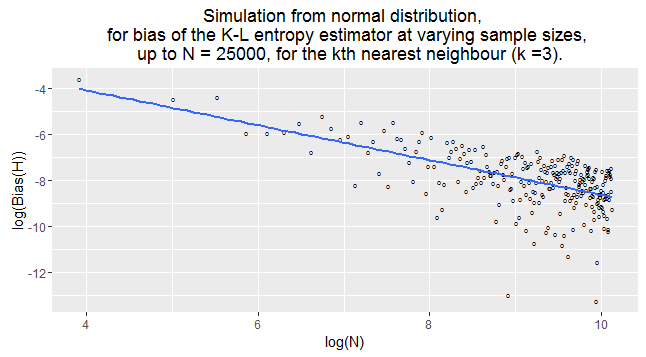
\includegraphics[width=\textwidth]{./Graphs/Normal_k=3_plot.png}
  \end{center}
\caption{Regression plot of $\log|Bias(\hat{H}_{N, 3})|$ against $\log(N)$}
  \label{normal_k=3_graph}
\end{figure}

The graph showing the relationship given by \ref{logbias} is shown in figure \ref{normal_k=3_graph}. The have found the coefficients for the formula \ref{bias}, for the graph shown with $k=3$ are given by $a_{3} = 0.6443$ and $c_{3} = 0.1156$, thus;
\begin{equation}
|Bias(\hat{H}_{N, 3})| \approx \frac{0.1156}{N^{0.6443}} \nonumber
\end{equation}
So for $N=50,000$, this implies that $|Bias(\hat{H}_{50000, 3})| \approx 0.000176$, which is close to the value found in table \ref{normal_k=3_table}, that $|Bias(\hat{H}_{50000, 3})| \approx 0.000085$. We here have that $a_{3} \geq a_{2} \geq a_{1}$, hence, according to this analysis, when $k=3$ we have a stronger negative relationship between the bias and $N$. A full comparison of the regression analysis for each $k$ is conducted in section \ref{N_compare_k}.




\subsubsection{k=5} \label{N_k=5}
Now we consider the estimator, shown in equation \ref{KLest}, for k=5. This takes the form;
\begin{equation}
\hat{H}_{N, 5} = \frac{1}{N} \sum_{i=1}^{N} log \left[ \frac{2\rho_{(5),i}(N-1)}{e^{\Psi(5)}} \right] \nonumber
\end{equation}

\begin{table}
\caption{1-dimensional normal distribution, $k=5$} \label{normal_k=5_table}
\begin{center}
\begin{tabular}{| l | c c c|} 
\toprule
$N$ & $\hat{H}_{N, 5}$ & $|Bias(\hat{H}_{N, 5})|$ & $Var(Bias(\hat{H}_{N, 5}))$ \\
\midrule[1pt]
100     & 1.391834     & 0.02710439666     & 0.00807261026  \\
200     & 1.405356     & 0.01358205942     & 0.00425419382  \\
500     & 1.411436     & 0.00750282472     & 0.00168848112  \\
1000    & 1.415091     & 0.00384740080     & 0.00091927735  \\
5000    & 1.418150     & 0.00078877480     & 0.00018941496  \\
10000   & 1.418648     & 0.00029099525     & 0.00008767553  \\
25000   & 1.418879     & 0.00005917171     & 0.00003243503  \\
50000   & 1.418644     & 0.00029451951     & 0.00001705529  \\
\hline
\end{tabular}
\end{center}
\end{table}

Comparing this to the exact entropy for the standard normal distribution, (\ref{normal_exact}), gives table \ref{normal_k=5_table}. Here, the $|Bias(\hat{H}_{N, 5})|$ decreases as $N$ goes from $100 \to 25,000$, but at $50,000$ this jumps to a larger number. Up to $25,000$ indicates that the estimator is becoming closer to the actual value, the jump at $50,000$  could be due to a number of reasons. 

Firstly, this could indicate that for $k=5$, this estimator becomes less efficient, and doesn't satisfy the property ...  as strongly as smaller values of $k$ have done so far. Secondly,this could just be an error in the data for $|Bias(\hat{H}_{50000, 5})|$ ; since we are only considering a relative small number of samples, 500, and are taking the average of this, we could just have an outlier. Lastly, there could be an error in the previous two data points, $|Bias(\hat{H}_{25000, 5})|$ and $|Bias(\hat{H}_{10000, 5})|$, causing us to either believe it is decreasing, when it isn't.

To determine the reason for this jump of Bias in the wrong direction, I will examine $|Bias(\hat{H}_{50000, 5})|$ for 3,000 samples and see if this is consistent with the previous findings. I have found this number to be; 
\begin{equation} 
|Bias(\hat{H}_{50000, 5})|  \approx 0.00006034936 \nonumber
\end{equation}
This gives us a much smaller bias than $|Bias(\hat{H}_{50000, 5})|$ shown in table \ref{normal_k=5_table}, however, this is still not smaller than the value of $|Bias(\hat{H}_{25000, 5})|$ shown in the same table. This could mean that for $k=5$, the estimator doesn't satisfy the consistency condition as strongly as the previous estimators for $k=1, 2, 3$.

However, if we consider the graph in figure \ref{normal_k=5_graph}, we can see an obvious negative relationship between the logarithm of $|Bias(\hat{H}_{N, 5})|$ and the logarithm of $N$. Henceforth, I would expect that the numbers above are within the standard error range, so that for $k=5$, we do have an estimator which satisfies the consistency condition, shown in Theorem \ref{consistency_theorem}.

\begin{figure}
  \begin{center}
    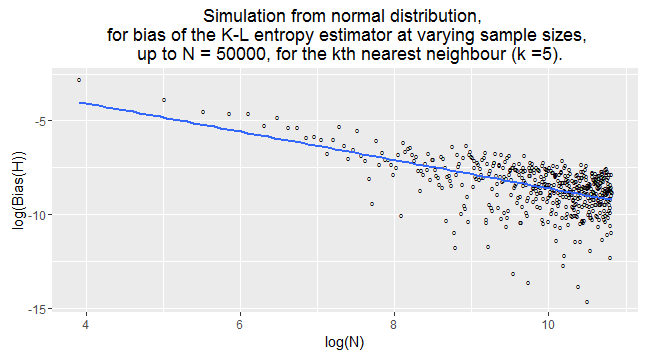
\includegraphics[width=\textwidth]{./Graphs/Normal_k=5_plot.png}
  \end{center} 
\caption{Regression plot of $\log|Bias(\hat{H}_{N, 5})|$ against $\log(N)$}
  \label{normal_k=5_graph}
\end{figure}

By plotting the graph in figure \ref{normal_k=5_graph}, we have found the coefficients for the formula \ref{bias}, for $k=5$, which are given by $a_{5} = 0.7568$ and $c_{5} = 0.3557$ , thus;
\begin{equation}
|Bias(\hat{H}_{N, 5})| \approx \frac{0.3557}{N^{0.7568}} \nonumber
\end{equation}
For these coefficients we have that $a_{5} \geq a_{3} \geq a_{2} \geq a_{1}$, thus according to this analysis, we have a stronger consistency of our estimator for $k=5$, in comparison to $k=1, 2, 3$. This comparison will be considered in more detail in section \ref{N_compare_k}.




\subsubsection{k=10} \label{N_k=10}
The last estimator for the entropy of a sample from the standard normal distribution that I wish to explore is that for $k=10$. Here, the estimator takes the form;
\begin{equation}
\hat{H}_{N, 10} = \frac{1}{N} \sum_{i=1}^{N} log \left[ \frac{2\rho_{(10),i}(N-1)}{e^{\Psi(10)}} \right] \nonumber
\end{equation}
The results for the comparison between this estimator and \ref{normal_exact} are displayed in table \ref{normal_k=10_table}.

\begin{table}
\caption{1-dimensional normal distribution, $k=10$} \label{normal_k=10_table}
\begin{center}
\begin{tabular}{| l | c c c|} 
\toprule
N & $\hat{H}_{N, 10}$ & $|Bias(\hat{H}_{N, 10})|$ & $Var(Bias(\hat{H}_{N, 10}))$ \\
\midrule[1pt]
100     & 1.375699     & 0.0432399931     & 0.00678770166  \\
200     & 1.391934     & 0.0270050257     & 0.00293164825  \\
500     & 1.407625     & 0.0113137866     & 0.00148669638  \\
1000    & 1.411684     & 0.0072549983     & 0.00067990485  \\
5000    & 1.417306     & 0.0016322988     & 0.00013650841  \\
10000   & 1.418196     & 0.0007429215     & 0.00006783354  \\
25000   & 1.418356     & 0.0005825702     & 0.00003162161  \\
50000   & 1.418790     & 0.0001488755     & 0.00001318863  \\
\hline
\end{tabular}
\end{center}
\end{table}

Here, we can again see that this estimator is satisfying the consistency condition, from Theorem \ref{consistency_theorem}, as $\hat{H}_{N, 10} \approx  0.0432 \to 0.0001$ as $N \approx 100 \to 50,000$. Comparing this to previous values of $k$, we can see that the bias changes decreases in a similar manner to that for $k=1, 2, 3$.

\begin{figure}
  \begin{center}
    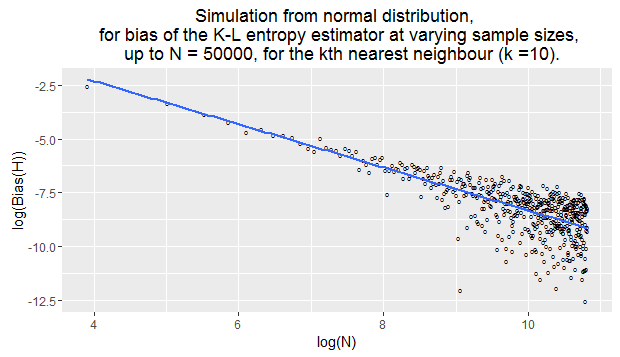
\includegraphics[width=\textwidth]{./Graphs/Normal_k=10_plot.png}
  \end{center}
\caption{Regression plot of $\log|Bias(\hat{H}_{N, 10})|$ against $\log(N)$}
  \label{normal_k=10_graph}
\end{figure}

From the graph in Figure \ref{normal_k=10_graph}, we have the relationship between the Bias and $N$ taking the form;
\begin{equation}
|Bias(\hat{H}_{N, 5})| \approx \frac{5.5942}{N^{1.0055}} \nonumber
\end{equation}
So we have the coefficients of the regression formula (\ref{bias}) as $a_{10} = 1.0055$ and $c_{k} = 5.5942$. These numbers are very contrasting to the previous coefficients that we have seen for the other values of $k$ in this distribution. This could indicate, either an error in the simulation, or that for $k=10$, the results are very different to that for the smaller values of $k$. I will explore this difference in more details in section \ref{N_compare_k}.




\subsubsection{Comparison of k} \label{N_compare_k}
The above analysis, sections \ref{N_k=1} to \ref{N_k=10} is done to examine the difference in the bias of the estimator for different values of k. Considering the above samples, for $N=25,000$ and $N=50,000$, we can create a table to compare the values of the bias of the estimator for the different values of $k$ considered;

\begin{table}
\caption{1-dimensional normal distribution, comparison of $k$} \label{normal_kcompare_table}
\begin{center}
\begin{tabular}{| l | c c c c|} 
\toprule
$k$ & $|Bias(\hat{H}_{25000, k})|$ & $Var(Bias(\hat{H}_{25000, k}))$ & $|Bias(\hat{H}_{50000, k})|$ & $Var(Bias(\hat{H}_{50000, k}) )$ \\
\midrule[1pt]
1    & 0.00006147045   & 0.0001088641     & 0.00034705584   & 0.0000496450   \\
2    & 0.0005620780     & 0.00005791073   & 0.0002574343     & 0.00002956529 \\
3    & 0.0001760980     & 0.00004286406   & 0.0000851863     & 0.00002257717 \\
5    & 0.00005917171   & 0.00003243503   & 0.00029451951   & 0.00001705529 \\
10  & 0.0005825702     & 0.00003162161   & 0.0001488755     & 0.00001318863 \\
\hline
\end{tabular}
\\[10pt]
\caption*{This table is comparing the values of $|Bias(\hat{H}_{N, k})|$ for the values of $k$ explored in tables \ref{normal_k=1_table}, \ref{normal_k=2_table}, \ref{normal_k=3_table}, \ref{normal_k=5_table} and  \ref{normal_k=10_table} with $N=25,000$ and $N=50,000$, when the estimator is taken over $500$ samples}
\end{center}
\end{table}

The results shown in table \ref{normal_kcompare_table} are inconclusive in determining if larger/smaller values of k generate better estimators, with smaller bias. However, these results are consistent in showing that for the larger value of N, the smaller the variance in the estimator. The results for the Bias are not conclusive; because, for $N=25,000$ we can see that with $k=1, 5$ and possibly $k=3$ have a slight smaller bias than the others. However, when $N=50,000$ we find that for $k=3, 10$ we have the smallest values of bias. These are inconsistent with one and other. To further examine this, I will now generate a table for values $k=1, 2, 3, 5, 10$ with $N=50,000$ in all cases. Moreover, this time I will consider $3,000$ samples of this size, not the $500$ considered before, and will find the mean and variance of the bias of this estimator.

\begin{table}
\caption{1-dimensional normal distribution, comparison of $k$} \label{normal_kcompare2_table}
\begin{center}
\begin{tabular}{| l | c c |} 
\toprule
$k$ &  $|Bias(\hat{H}_{50000, k})|$ & $Var(Bias(\hat{H}_{50000, k}))$ \\
\midrule[1pt]
1      & 0.00013495546     & 0.00005116758  \\
2      & 0.00012647214     & 0.00002868082  \\
3      & 0.00003478968     & 0.00002299754  \\
5      & 0.00006034936     & 0.00001733369  \\
10    & 0.00022455715     & 0.00001409080  \\
\hline
\end{tabular}
\\[10pt]
\caption*{This table is comparing the values of $|Bias(\hat{H}_{N, k})|$ for the values of $k$ explored before now with only $N=50,000$ and the estimator being taken over $3,000$ samples}
\end{center}
\end{table}

The results in table \ref{normal_kcompare2_table}, consider the scenario set out above, and we can see that $|Bias(\hat{H}_{N, k})|$ is the smallest, for sample size $N=50,000$, when $k=3$, which is consistent with the results found in table \ref{normal_kcompare_table}. So from these simulations, we can conclude that for large $N$, the consistency condition is best satisfied when $k=3$. Interestingly, the $Var(Bias(\hat{H}_{50000, k})) \to 0$ for $k \to 10$, but this is to be expected, as by the definition of the estimator using the nearest neighbour method. Taking a larger $k$ in the nearest neighbour method will produce less varied results, this is because more smoothing takes place for a larger $k$, eventually - if $k$ is made large enough - the output will be constant and the variance negligible regardless of the inputted values. Thus, considering the variance of the bias of the estimator is not necessarily informative.

\begin{table}
\caption{Comparison of coefficients of regression $a_{k}$ and $c_{k}$ from equation \ref{bias}, for 1-dimensional normal distribution} \label{normal_a_c_compare_table}
\begin{center}
\begin{tabular}{| l | l l |} 
\toprule
$k$ &  $a_{k}$ & $c_{k}$ \\
\midrule[1pt]
1      & 0.4594     & 0.0249  \\
2      & 0.5998     & 0.0746  \\
3      & 0.6443     & 0.1156  \\
5      & 0.7568     & 0.3557  \\
10    & 1.0055     & 5.5942  \\
\hline
\end{tabular}
\\[10pt]
\end{center}
\end{table}

Table \ref{normal_a_c_compare_table}, shows that as $k$ runs from $1 \to 10$, we have that $a_{k}$ and $c_{k}$ both increase, with a large jump between $k=5$ and $k=10$. The higher the value of $a_{k}$, the stronger the negative relationship is between the two variables in question, so for a larger values of $a_{k}$, we have that $|Bias(\hat{H}_{N, k})| \to 0$ for large $N$ faster than smaller values of $a_{k}$. This is due to the relationship between $|Bias(\hat{H}_{N, k})|$ and $a_{k}$ shown in equation (\ref{bias}). Thus, considering a large sample size, say $N=100,000$, we can find the bias of the Kozachenko-Leonenko estimator according to the regressional relationship for each $k$; $|Bias(\hat{H}_{N, k})| = \frac{c_{k}}{N^{a_{k}}}$. We find that;
\begin{gather*}
|Bias(\hat{H}_{100000, 1})| \approx  \frac{0.0249}{100000^{0.4594}}   \approx 0.00012566 \\
|Bias(\hat{H}_{100000, 2})| \approx  \frac{0.0746}{100000^{0.5998}}   \approx 0.00007477 \\
|Bias(\hat{H}_{100000, 3})| \approx  \frac{0.1156}{100000^{0.6443}}   \approx 0.00006942 \\
|Bias(\hat{H}_{100000, 5})| \approx  \frac{0.3557}{100000^{0.7568}}   \approx 0.00005949 \\
|Bias(\hat{H}_{100000, 10})| \approx  \frac{5.5942}{100000^{1.10055}}   \approx 0.00005251 
\end{gather*}

This shows that the bias decreases slightly faster for a higher values of $k$. I have also compared these relationships through a graph of the regression lines found from plotting the simulations above, shown in Figure \ref{normal_comparison_graph}. Moreover, I have plotted the actual lines for the relationship between $|Bias(\hat{H}_{N, k})|$ and $N$, using the relationship shown in equation (\ref{bias}), this shows that ... TODO.

\begin{figure}
  \begin{center}
    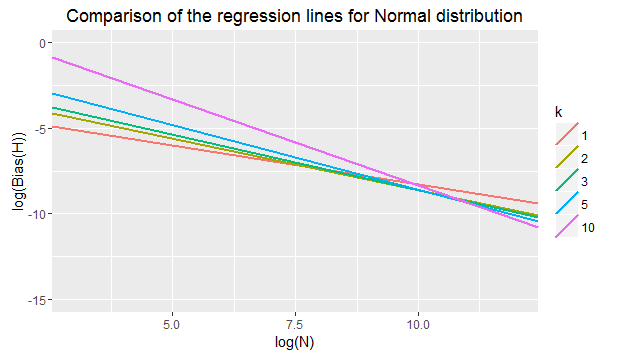
\includegraphics[width=\textwidth]{./Graphs/Normal_comparison.png}
  \end{center}
\caption{Plot of regression lines for $\log|Bias(\hat{H}_{N, k})|$ against $\log(N)$, for $k=1, 2, 3, 5, 10$, for samples from the normal distribution}
  \label{normal_comparison_graph}
\end{figure}

I have also considered a plot of the values of $a_{k}$ and $c_{k}$ against $k$, to see if there is a clear relationship between the value of $k$ and the coefficients, $a$ and $c$. This shows that ... TODO

TODO .. add in plots 





\subsection{1-dimensional Uniform distribution}

I will now explore the entropy of samples from the 1-dimensional uniform distribution, $U[a b]$. This distribution also has an exact formula to work out the entropy for. We can find this formula by considering the density function, $f$, from the uniform distribution, which is given by;
\[
f(x) =  \begin{cases} 
      \frac{1}{b-a} & a \leq x \leq b \\
      0 & otherwise
   \end{cases}
\]
Using the definition of Shannon entropy given in equation (\ref{ShaEnt}), we can find the exact entropy for the uniform distribution;
\begin{align*}
H &= - \int_{x : f(x) > 0} f(x) log(f(x)) dx \\ 
&= - \int_{a}^{b} \frac{1}{b-a} log \left[ \frac{1}{b-a} \right] dx  \\
&= - \frac{1}{b-a} log \left[ \frac{1}{b-a} \right]  \int_{a}^{b} dx  \\
&= -  log  \left[ \frac{1}{b-a} \right] 
\end{align*}
Thus, the actual value of entropy for the uniform distribution is given by;
\begin{equation} \label{UnifEnt}
H = log [ b-a ]
\end{equation}

The uniform distribution automatically satisfies the conditions .... because ... 

In our samples we will be consider the uniform distribution $U[0,100]$; this is because, using the standard uniform, $U[0,1]$, would fail since taking $N=50,000$ samples between 0 and 1 would generate problems as the pdf would be $f(x) = 1 , \quad 0 \leq x \leq 1$, which would incur working on a very small scale; i.e taking a points with distance between them as $\approx 0.00002$ along the x-direction. Thus, I will be using the pdf $f(x) = 0.01 , \quad 0 \leq x \leq 100$, which gives the exact entropy to be;
\begin{equation} \label{uniform_exact}
H = log(100) \approx 4.605170
\end{equation}

Similarly to the 1-dimensional normal distribution, we have for the 1-dimensional uniform distribution that $d=1$ so $V_{1} = 2$, thus our estimator takes the form of equation (\ref{KLest_d=1});
\begin{equation}
\hat{H}_{N, k} =  \frac{1}{N} \sum_{i=1}^{N} log \left[ \frac{2\rho_{(k),i}(N-1)}{e^{\Psi(k)}} \right]\nonumber
\end{equation}




\subsubsection{k=1} \label{U_k=1}
We will begin by considering 500 samples from the uniform distribution $U[0,100]$, of size $N=100 \to 50,000$ and finding the estimator for $k=1$, which is of the form;
\begin{equation} 
\hat{H}_{N, 1} = \frac{1}{N} \sum_{i=1}^{N} log \left[ \frac{2\rho_{(1),i} (N-1)}{e^{-\gamma}} \right] \nonumber
\end{equation}
Considering the bias for this estimator against the actual value (\ref{uniform_exact}) for different samples sizes $N$ gives Table \ref{uniform_k=1_table}.

\begin{table}
\caption{1-dimensional uniform distribution, $k=1$} \label{uniform_k=1_table}
\begin{center}
\begin{tabular}{| l | c c c|} 
\toprule
N & $\hat{H}_{N, 1}$ & $|Bias(\hat{H}_{N, 1})|$ & $Var(Bias(\hat{H}_{N, 1}))$ \\
\midrule[1pt]
100     & 4.600031     & 0.0051387799     & 0.02082714731  \\
200     & 4.610892     & 0.0057214665     & 0.01051097236  \\
500     & 4.606304     & 0.0011339740     & 0.00464501181  \\
1000    & 4.604414     & 0.0007562145     & 0.00197979118  \\
5000    & 4.606068     & 0.0008976195     & 0.00041910068  \\
10000   & 4.604871     & 0.0002993139     & 0.00021349464  \\
25000   & 4.605529     & 0.0003587332     & 0.00008599342  \\
50000   & 4.605547     & 0.0003764863     & 0.00004437685  \\
\hline
\end{tabular}
\end{center}
\end{table}

From table \ref{uniform_k=1_table} there is an obvious decrease in value of the Bias, for larger $N$, with $|Bias(\hat{H}_{N, 1})|$ decreasing from $\approx 0.005$ to $\approx 0.0004$. This decrease is similar to that considered in the normal distribution for $k=1$, where $|Bias(\hat{H}_{N, 1})|$ went from $\approx 0.01$ to $\approx 0.0003$; however, the difference is that for this distribution, the estimator seems to be more accurate for smaller $N$. Another thing to notice from this table is that, even through there is a general decrease, considering each rows in the table in comparison to the next does not necessarily show a decrease. The smallest value of bias occurs for $N=10,000$, which does not correspond with the findings for the normal distribution. This could indicate a number of features;

\begin{itemize}
\item The values in table \ref{uniform_k=1_table} contains outliers - this could be the case, since the numbers seem to jump around more ion this occasion than any others seen before. However, for $k=1$ the bias decreases from $0.0057 \to 0.00029$ in the uniform distribution and decreases from $0.013 \to 0.00034$ in the normal distribution (not necessarily as $N$ gets larger); these values of bias are not too dissimilar from one and other. Also, the tables are made from considering $500$ samples of each $N$, finding the estimator in all cases, then taking the average of these as the actual estimator; this makes an outlier much less likely, as they would have been smoothed out from the averaging process.

\item The actual value of entropy is significantly smaller itself, so the bias of the estimator is accordingly small - this is again unlikely, since the actual value of entropy for the uniform distribution is given by $\approx 4.605170$ (\ref{uniform_exact}), and the for the normal distribution is $\approx 1.418939$ (\ref{normal_exact}). These values are not significantly different to one and other, also under this reasoning, one would expect the normal distribution to have an accordingly smaller bias than the uniform - but we are experiencing values the other way around.

\item The estimator works better for samples from uniform than the normal distributions - this should not be true since the uniform distribution satisfies the conditions under which this estimator can be used in exactly the same manner as the normal distribution, so one would not expect samples from a specific distribution to yield a more accurate estimator for entropy. However, this is the most likely reason for the difference occurring between the two distributions. This is due to, as mentioned before, the nature of the uniform distribution, that by using $U[0, 100]$, for $N=50,000$ each sample would be $\approx 0.002$ distance apart. So using the nearest neighbour method; all of the data in the samples will have close neighbours, which could be the reason for the unreliable values shown in table \ref{uniform_k=1_table}.
\end{itemize}

To understand what is occurring in table \ref{uniform_k=1_table}, I have plotted the results of the approximate correlation between the bias of the estimator against $N$, as shown in equation \ref{logbias}. This is shown in Figure \ref{uniform_k=1_graph}.

\begin{figure}
  \begin{center}
    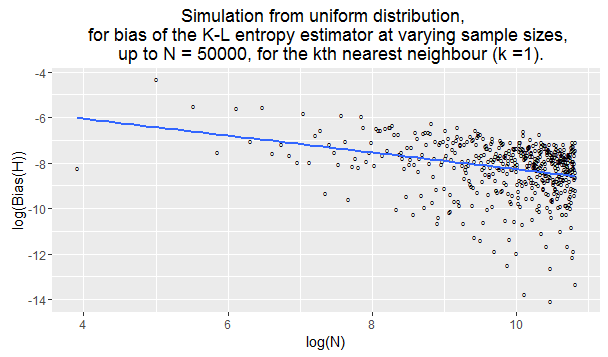
\includegraphics[width=\textwidth]{./Graphs/Uniform_k=1_plot.png}
  \end{center}
\caption{Regression plot of $\log|Bias(\hat{H}_{N, 1})|$ against $\log(N)$}
  \label{uniform_k=1_graph}
\end{figure}

 From this analysis, the bias of the Koazchenko-Leonenko estimator for entropy has the following relationship with $N$;
\begin{equation}
|Bias(\hat{H}_{N, 2})| \approx \frac{0.0103}{N^{0.3698}}\nonumber
\end{equation}
TODO.. write about this and plot graph for k=1 and regression coefs + comparison to the normal distribution
a
[1] 0.3698

c
[1] 0.0103





\subsubsection{k=2} \label{U_k=2}
We now wish to consider the estimator for $k=2$, which takes the form;
\begin{equation} 
\hat{H}_{N, 1} = \frac{1}{N} \sum_{i=1}^{N} log \left[ \frac{2\rho_{(1),i} (N-1)}{e^{-\gamma + 1}} \right] \nonumber
\end{equation}

\begin{table}
\caption{1-dimensional uniform distribution, $k=2$} \label{uniform_k=2_table}
\begin{center}
\begin{tabular}{| l | c c c|} 
\toprule
N & $\hat{H}_{N, 2}$ & $|Bias(\hat{H}_{N, 2})|$ & $Var(Bias(\hat{H}_{N, 2}))$ \\
\midrule[1pt]
100     & 4.606725     & 0.0015545396     & 0.00851906912  \\
200     & 4.610785     & 0.0056145269     & 0.00456819154  \\
500     & 4.611599     & 0.0064290000     & 0.00189878458  \\
1000    & 4.603534     & 0.0016366244     & 0.00095980274  \\
5000    & 4.604978     & 0.0001921979     & 0.00017282038  \\
10000   & 4.605488     & 0.0003180407     & 0.00009978981  \\
25000   & 4.604753     & 0.0004176853     & 0.00004003515  \\
50000   & 4.605480     & 0.0003095010     & 0.00001737807  \\
\hline
\end{tabular}
\end{center}
\end{table}

Using the same parameters as before; taking $500$ samples of size $N=100 \to 50,000$ from the uniform, $U[0, 100]$, distribution, we get the results in Table \ref{uniform_k=2_table}. These show that there is a general decrease in bias for a larger $N$ from $|Bias(\hat{H}_{500, 2})| \approx  0.006430$ to $|Bias(\hat{H}_{50000, 2})| \approx 0.00031$; however, if we look closely, in a similar fashion to for $k=1$, the bias is not always decreasing as $N$ gets larger. This is shown in it increasing for the first 3 data points; $N=100, 200 ,500$, then decreasing for a bit, then increasing again for $N = 10000, 25000$. The smallest value of Bias actually occurs at $N=5000$, which does not correspond with the results one would expect from this analysis. Moreover, the size of the bias does begin smaller for this case than it has done previously for values from the normal distribution, section \ref{Normal_d=1}. 

To understand better what is occurring in table \ref{uniform_k=2_table}, I have plotted the results of the approximate correlation between the bias of the estimator against $N$, as shown in equation \ref{bias}. This is shown in Figure \ref{uniform_k=2_graph}.

\begin{figure}
  \begin{center}
    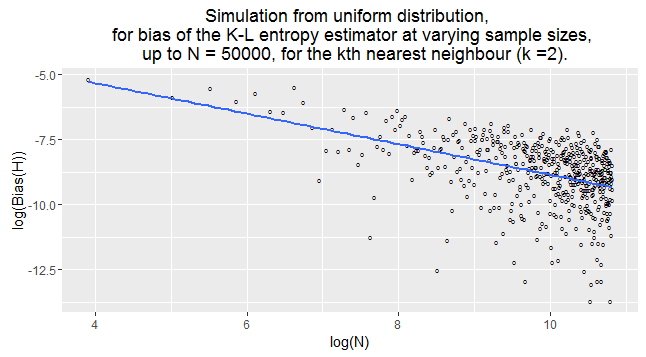
\includegraphics[width=\textwidth]{./Graphs/Uniform_k=2_plot.png}
  \end{center}
\caption{Regression plot of $\log|Bias(\hat{H}_{N, 2})|$ against $\log(N)$}
  \label{uniform_k=2_graph}
\end{figure}

This graph has the regression line plotted of the form \ref{logbias}, with $a_{2} \approx 0.5857$ and $c_{2} \approx 0.00503$. From this analysis, I would expect the bias of the Koazchenko-Leonenko estimator for entropy to have the following relationship with $N$;
\begin{equation}
|Bias(\hat{H}_{N, 2})| \approx \frac{0.0503}{N^{0.5857}}\nonumber
\end{equation}
As we can see from the graph, the relationship is obviously a negative correlation, and the values around the line are sparsely located. So I believe the reason for table \ref{uniform_k=2_table} not looking as expected, is just due to bad luck in the values of $N$ that I have chosen to be numerically represented in it. The graph plotted and the regression coefficients, align well with the normal distribution. Thus removing any uncertainty that we have about the estimator of entropy for a sample from the uniform distribution acting differently to that from the normal distribution. A comparison of the values of $a_{2}$ and $c_{2}$, with other values of $k$, will be further explored in section \ref{U_compare_k}.



\subsubsection{k=3} \label{U_k=3}
We now wish to consider the estimator for $k=3$, which takes the form;
\begin{equation} 
\hat{H}_{N, 1} = \frac{1}{N} \sum_{i=1}^{N} log \left[ \frac{2\rho_{(1),i} (N-1)}{e^{-\gamma + \frac{3}{2}}} \right] \nonumber
\end{equation}

Using the same parameters as before; taking $500$ samples of size $N=100 \to 50,000$ from the uniform, $U[0, 100]$, distribution, we get the results in Table \ref{uniform_k=3_table}. These results are again inconclusive, to showing a the consistency condition that $|Bias(\hat{H}_{N, 3})| \to 0$ as $N \to \infty$, since the numbers jump around and increase between, say $N=500$ and $1000$, which we would not expect to happen.

\begin{table}
\caption{1-dimensional uniform distribution, $k=3$} \label{uniform_k=3_table}
\begin{center}
\begin{tabular}{| l | c c c|} 
\toprule
N & $\hat{H}_{N, 3}$ & $|Bias(\hat{H}_{N, 3})|$ & $Var(Bias(\hat{H}_{N, 3}))$ \\
\midrule[1pt]
100     & 4.610386     & 0.00521552744     & 0.00697968570  \\
200     & 4.611047     & 0.00587685467     & 0.00316173901  \\
500     & 4.605035     & 0.00013506468     & 0.00121563168  \\
1000    & 4.606418     & 0.00124808620     & 0.00054151215  \\
5000    & 4.605270     & 0.00009934301     & 0.00011448612  \\
10000   & 4.604869     & 0.00030102035     & 0.00007028042  \\
25000   & 4.605341     & 0.00017121288     & 0.00002543334  \\
50000   & 4.605123     & 0.00004761182     & 0.00001155187  \\
\hline
\end{tabular}
\end{center}
\end{table}

I believe that the best way to show this consistency condition is to just consider the graphical representation, and to not worry about the tabulated values, as they're inconsistent due to the reasons stated in section \ref{U_k=2}. From this plot, Figure \ref{uniform_k=3_graph}, I have found that $a_{3} \approx 0.6291$ and $c_{3} \approx 0.0737$. This implies the relationship;
\begin{equation}
|Bias(\hat{H}_{N, 3})| \approx \frac{0.0737}{N^{0.6291}}\nonumber
\end{equation}
In comparison to this, for $k=2$, we had that $a_{2} \approx 0.5857$, so $a_{2} < a_{3}$, which implies that the relationship for $k=3$ is stronger than that for $k=2$. A more detailed comparison will be further explored in section \ref{U_compare_k}.

\begin{figure}
  \begin{center}
    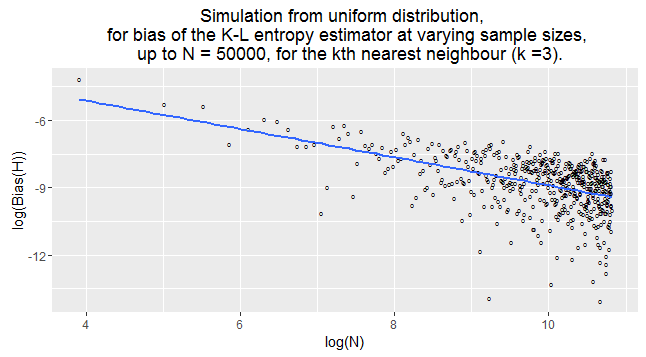
\includegraphics[width=\textwidth]{./Graphs/Uniform_k=3_plot.png}
  \end{center}
\caption{Regression plot of $\log|Bias(\hat{H}_{N, 3})|$ against $\log(N)$}
  \label{uniform_k=3_graph}
\end{figure}


\subsubsection{k=5} \label{U_k=5}
Now we consider the estimator, shown in equation \ref{KLest}, for k=5. This takes the form;
\begin{equation}
\hat{H}_{N, 5} = \frac{1}{N} \sum_{i=1}^{N} log \left[ \frac{2\rho_{(5),i}(N-1)}{e^{\Psi(5)}} \right] \nonumber
\end{equation}

Comparing this estimator to the exact value of entropy, shown in equation (\ref{uniform_exact}), for 500 samples of size $N$, as before, we get an inconclusive result from table \ref{uniform_k=5_table}. This is again due to the fact that taking a larger number of samples around a relatively small interval, will give similar results; hence, the relationship is again not as obvious from this. 

\begin{table}
\caption{1-dimensional uniform distribution, $k=5$} \label{uniform_k=5_table}
\begin{center}
\begin{tabular}{| l | c c c|} 
\toprule
N & $\hat{H}_{N, 5}$ & $|Bias(\hat{H}_{N, 5})|$ & $Var(Bias(\hat{H}_{N, 5}))$ \\
\midrule[1pt]
100     & 4.621001     & 0.0158306351     & 0.003899909770  \\
200     & 4.612364     & 0.0071935784     & 0.001744887954  \\
500     & 4.609793     & 0.0046227604     & 0.000768266967  \\
1000    & 4.607499     & 0.0023291487     & 0.000381576396  \\
5000    & 4.605980     & 0.0008102069     & 0.000068805987  \\
10000   & 4.606053     & 0.0008829085     & 0.000035434958  \\
25000   & 4.605339     & 0.0001689148     & 0.000015449454  \\
50000   & 4.605333     & 0.0001629615     & 0.000007555981  \\
\hline
\end{tabular}
\end{center}
\end{table}

Furthermore, I have considered a plot to represent equation (\ref{logbias}), shown in Figure \ref{uniform_k=5_graph}, where I have also found the coefficients of regression to be; $a_{5} \approx 0.7501$ and $c_{5} \approx 0.1889$. Thus, here we get the relationship;
\begin{equation}
|Bias(\hat{H}_{N, 5})| \approx \frac{0.1889}{N^{0.7501}}\nonumber
\end{equation}
In comparison to the previous two plots, we find that $a_{2} < a_{3} < a_{5}$, indicating that as $k$ increases the strength of the relationship between the $|Bias(\hat{H}_{N, k})|$ and $N$ also increases. This implies that $|Bias(\hat{H}_{N, k})| \to 0$ as $N \to \infty$ faster for $k=5$, over a smaller $k$. We can also see that $c_{k}$, so far, has also been increasing for larger $k \leq 5$. A comparison will be further explored in section \ref{U_compare_k}.

\begin{figure}
  \begin{center}
    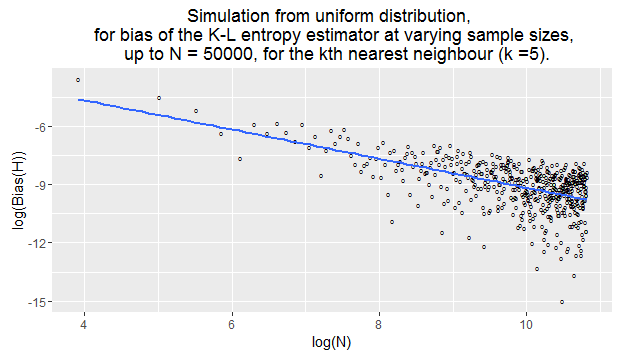
\includegraphics[width=\textwidth]{./Graphs/Uniform_k=5_plot.png}
  \end{center}
\caption{Regression plot of $\log|Bias(\hat{H}_{N, 5})|$ against $\log(N)$}
  \label{uniform_k=5_graph}
\end{figure}




\subsubsection{k=10} \label{U_k=10}
The last estimator for the entropy of a sample from the 1-dimensional uniform distribution that I wish to explore is that for $k=10$. Here, the estimator takes the form;
\begin{equation}
\hat{H}_{N, 10} = \frac{1}{N} \sum_{i=1}^{N} log \left[ \frac{2\rho_{(10),i}(N-1)}{e^{\Psi(10)}} \right] \nonumber
\end{equation}
The results for the comparison between this estimator and \ref{uniform_exact} are displayed in table \ref{uniform_k=10_table}.

\begin{table}
\caption{1-dimensional uniform distribution, $k=10$} \label{uniform_k=10_table}
\begin{center}
\begin{tabular}{| l | c c c|} 
\toprule
N & $\hat{H}_{N, 10}$ & $|Bias(\hat{H}_{N, 10})|$ & $Var(Bias(\hat{H}_{N, 10}))$ \\
\midrule[1pt]
100     & 4.639476     & 0.03430601671     & 0.002521145015  \\
200     & 4.621455     & 0.01628474750     & 0.000951343553  \\
500     & 4.611200     & 0.00602956738     & 0.000380048902  \\
1000    & 4.609219     & 0.00404887162     & 0.000186210819  \\
5000    & 4.605507     & 0.00033726494     & 0.000037485008  \\
10000   & 4.605341     & 0.00017035096     & 0.000018679424  \\
25000   & 4.605138     & 0.00003191065     & 0.000007044257  \\
50000   & 4.605190     & 0.00002025184     & 0.000003429152  \\
\hline
\end{tabular}
\end{center}
\end{table}

In comparison to what we have seen before in tables \ref{uniform_k=2_table}, \ref{uniform_k=3_table} and \ref{uniform_k=5_table}, we here have more of a obvious comparison, shown numerically, between the size of the sample, $N$, and the size of the bias. This fits in with the consistency condition from Theorem \ref{consistency_theorem}, that $|Bias(\hat{H}_{N, 10})| \to 0$ as $N \to \infty$. 

\begin{figure}
  \begin{center}
    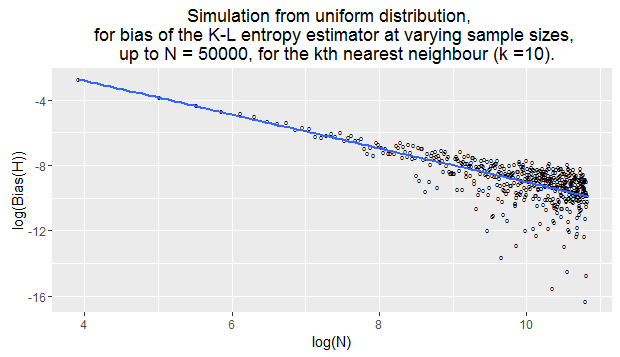
\includegraphics[width=\textwidth]{./Graphs/Uniform_k=10_plot.png}
  \end{center}
\caption{Regression plot of $\log|Bias(\hat{H}_{N, 10})|$ against $\log(N)$}
  \label{uniform_k=10_graph}
\end{figure}

TODO ..  graphical comparison.
a
[1] 1.0357
c
[1] 3.8217



\subsubsection{Comparison of k} \label{U_compare_k}
In sections \ref{U_k=1} to \ref{U_k=10}, I have explored the Koazchenko-Leonenko estimator for samples from the 1-dimensional uniform distribution. In the most part, the tables of information from this estimator were inconsistent and inconclusive, due to the nature of the uniform distribution; that the samples are very close to one and other. Because of this, I will not be going into more detail of that comparison; thus, will be focusing solely on the relationship shown in equation (\ref{bias});
\begin{equation}
|Bias(\hat{H}_{N, k})| = \frac{c_{k}}{N^{a_{k}}} \nonumber
\end{equation}
The results from the investigation above have been condensed into table \ref{uniform_k_comparison_table}, showing the change in values of $a_{k}$ and $c_{k}$ for different {k}.

\begin{table}
\caption{1-dimensional uniform distribution, a comparison of $k$} \label{uniform_k_comparison_table}
\begin{center}
\begin{tabular}{| l | c c|} 
\toprule
k & $a_{k}$ & $c{k}$ \\
\midrule[1pt]
1 & 0.3698 & 0.0103 \\
2 & 0.5857 & 0.0503 \\
3 & 0.6291 & 0.0737 \\
5 & 0.7501 & 0.1889 \\
10 & 1.0357 &  3.8217 \\
\hline
\end{tabular}
\end{center}
\end{table}

From table \ref{uniform_k_comparison_table}, we can see that as $k$ in creases from $1$ to $10$, that both $a_{k}$ and $c_{k}$ also increase. The value of $a_{k}$ increasing implies an increase in strength of the consistency condition, Theorem \ref{consistency_theorem};  $N (H - \mathbb{E}{\hat{H}_{N, k}})^2 \to 0 \quad  (N \to \infty)$, which is equivalent to saying that $|Bias(\hat{H}_{N, k})| \to 0 \quad (N \to \infty)$. Thus, considering a large sample size, say $N=100,000$, we can find the bias of the Kozachenko-Leonenko estimator according to the regressional relationship for each $k$;
\begin{gather*}
|Bias(\hat{H}_{100000, 1})| \approx  \frac{}{100000^{}}   \approx  \\
|Bias(\hat{H}_{100000, 2})| \approx  \frac{0.0503}{100000^{0.5857}}   \approx 0.000059301 \\
|Bias(\hat{H}_{100000, 3})| \approx  \frac{0.0737}{100000^{0.6291}}   \approx 0.000052719 \\
|Bias(\hat{H}_{100000, 5})| \approx  \frac{0.1889}{100000^{0.7501}}   \approx 0.000033553\\
|Bias(\hat{H}_{100000, 10})| \approx  \frac{3.8217}{100000^{1.0357}}  \approx 0.000025337
\end{gather*}
These values confirm our original thoughts that the larger value of $k \leq 10$ gives a more consistent estimator. Moreover, we can compare these values to those found for the standard normal distribution, along with comparing the values of $a_{k}$ and $c_{k}$, to see if the estimator has a similar accuracy for both distributions, this comparison is shown in table \ref{uniform_normal_comparison_table}.
In this comparison we can see that, the values of $a_{k}$ and $|Bias(\hat{H}_{100000, k})|$ are similar for both distributions, with $a_{k}$ varying by less that $\approx 0.015$ and $|Bias(\hat{H}_{100000, k})|$ varying by less than $\approx 0.000015$. Both of these confirm that the approximation to the relationship between the estimator and the actual value of entropy, is a good approximation to make; one which is consistent through both distributions considered so far.

\begin{table}
\caption{Comparison between 1-dimensional Uniform and Normal distribution} \label{uniform_normal_comparison_table}
\begin{center}
\begin{tabular}{| l | c c c | c c c |}
\toprule
{ |} &  \multicolumn{3}{c |}{Normal} & \multicolumn{3}{c |}{Uniform}\\
\hline
$k$   &  $a_{k}$  &  $c_{k}$  &  $|Bias(\hat{H}_{100000, k})|$  &  $a_{k}$  &  $c_{k}$  &  $|Bias(\hat{H}_{100000, k})|$  \\
\midrule[1pt]
1      & 0.4594     & 0.0249 &  0.00012566  &  &  & \\
2      & 0.5998     & 0.0746 &  0.00007477  &  0.5857  &  0.0503  &  0.000059301 \\
3      & 0.6443     & 0.1156 &  0.00006942  &  0.6291  &  0.0737  &  0.000052719 \\
5      & 0.7568     & 0.3557 &  0.00005949  &  0.7501  &  0.1889  &  0.000033553 \\
10    & 1.0055     & 5.5942 &  0.00005251  &  1.0357  &  3.8217  &  0.000025337 \\
\hline
\end{tabular}
\end{center}
\end{table}

Another comparison that we can make, is by considering the plot of the regression lines for the logarithm of  $|Bias(\hat{H}_{N, k})|$ against the logarithm of $N$, this relationship is shown in Figure \ref{?}. TODO .. plot this graph and talk about it

\begin{figure}
  \begin{center}
    \includegraphics[width=\textwidth]{./Graphs/Uniform_comparison.png}
  \end{center}
\caption{Plot of regression lines for $\log|Bias(\hat{H}_{N, k})|$ against $\log(N)$, for $k=1, 2, 3, 5, 10$, for samples from the uniform distribution}
  \label{uniform_comparison_graph}
\end{figure}


TODO.. plot a graph with regression lines for both the normal and uniform on top of one and other, discuss



\subsection{1-dimensional Exponential Distribution}

I will now be looking at the entropy of samples from the exponential distribution $exp(\lambda)$, where $\lambda > 0$ is the rate or inverse scale parameter. In a similar fashion to the previous distributions, the exponential also has an exact formula for the entropy, given the rate parameter $\lambda$. Using equation (\ref{ShaEnt}) and the density function for the exponential distribution $f(x) = \lambda e^{-\lambda x}$ for $x \in [0, \infty)$, we can write the exact entropy;
\begin{align*}
H &= - \int_{x : f(x) > 0} f(x) log(f(x)) dx \\ 
&= - \int_{0}^{\infty} \lambda e^{-\lambda x} log [ \lambda e^{-\lambda x} ] dx  \\
&= - \lambda \int_{0}^{\infty} \lambda e^{-\lambda x} [log(\lambda) - \lambda x] dx  \\
&= \lambda \int_{0}^{\infty} \lambda e^{-\lambda x} - log(\lambda) e^{-\lambda x} dx \\
&= - \lambda \left[x e^{-\lambda x}\right]_{0}^{\infty} + \int_{0}^{\infty}\lambda e^{-\lambda x} dx + log(\lambda) \left[ e^{-\lambda x}\right]_{0}^{\infty} \\
&= 0 + (log(\lambda) - 1) \left[e^{-\lambda x} \right]_{0}^{\infty} \\
&= -(log(\lambda) - 1)
\end{align*}

Thus we have the the exact value of entropy for the exponential distribution, given the rate parameter $\lambda > 0$, is;
\begin{equation} \label{ExpEnt}
H = 1 - log(\lambda)
\end{equation}

I have decided to choose to explore the exponential distribution with rate parameter $\lambda = 0.5$, this is because, if I choose $\lambda > e \approx 2.7183$ we get a negative values of entropy, $H < 0$, which will introduce problems when considering the modulus of the bias; hence, for this analysis it will be more beneficial to consider a positive value of entropy, $H$. Also, for $\lambda \geq 1$, we have a small value of entropy, which would cause problems when calculating large samples and their entropy. Therefore, I have chosen a random number for the rate parameter such that $\lambda \in (0, 1)$, so for this value of $\lambda=0.5$, the exact entropy is given by;
\begin{equation} \label{exponential_exact}
H = 1 - log(0.5) \approx 1.693147
\end{equation}
Moreover, I am again considering a 1-dimensional distribution; thus $V_{d} = V_{1} = 2$, and;
\begin{equation}
\hat{H}_{N, k} =  \frac{1}{N} \sum_{i=1}^{N} log \left[ \frac{2\rho_{(k),i}(N-1)}{e^{\Psi(k)}} \right]\nonumber
\end{equation}
is the form of the Kozachenko-Leonenko estimator that I will be considering here.



\subsubsection{k=1} \label{E_k=1}


a
[1] 0.0001

c
[1] 1.6947



\end{document}